\chapter{System Design}\label{chap:systemDesign}

This chapter describes the main content of our research. We begin by providing an overview of the problem our system is trying to solve, define components necessary for understanding this problem, and explain the scope of this problem we specifically tackle and why. We then present an overview of the successor algorithm we have created to attempt to solve this problem, before going into more depth on each the components of this algorithm, including details on their implementation. This includes the Monte Carlo Tree Search (MCTS) algorithm and how it has been integrated into IMPSY, our use of parameter based state representation to build a novel heuristic, and the parameters we have developed to integrate into this heuristic. Videos of the performances using the system, which are also used in our evaluation, as well as the code for the system, can be found on Github\footnote{\url{https://github.com/squatter1/impsy}}

\section{Problem Formulation}
It is important to clearly define the problem this system is trying to solve in a more formal manner than previously, before explaining the system itself. We build our work on top of the musical prediction system IMPSY~\cite{Martin2019IMPSY}, which is a system that uses a MDRNN to produce a GMM of possible next notes, with this GMM being randomly sampled from to produce a note. We are specifically interested in the call and response mode of IMPSY, where the user performs for a period of time, and then when the user stops, the system takes over and aims to predictively continue on from where the user left off. When the system takes over, the MDRNN prediction algorithm is triggered. The input for this MDRNN algorithm is the previous control input played, which is an $n$ dimensional vector representing the state of control parameters for an instrument, necessarily including a time dimension representing the length of time between this control input and when the next control input should happen. The input state also implicitly includes memory of previous control inputs through the LSTM RNN architecture. The output of the MDRNN is a random sample from an $n$ dimensional GMM, with any sample from the GMM representing a control input for the instrument. Our problem formulation is the same as with IMPSY, with our only goal being to improve the prediction process, not to fundamentally change the functionality of IMPSY. Figure~\ref{fig:IMPSY} shows the original IMPSY prediction system, and Figure~\ref{fig:Successor} highlights how our prediction system incorporates and expands upon this. 

\begin{figure}[th!]
    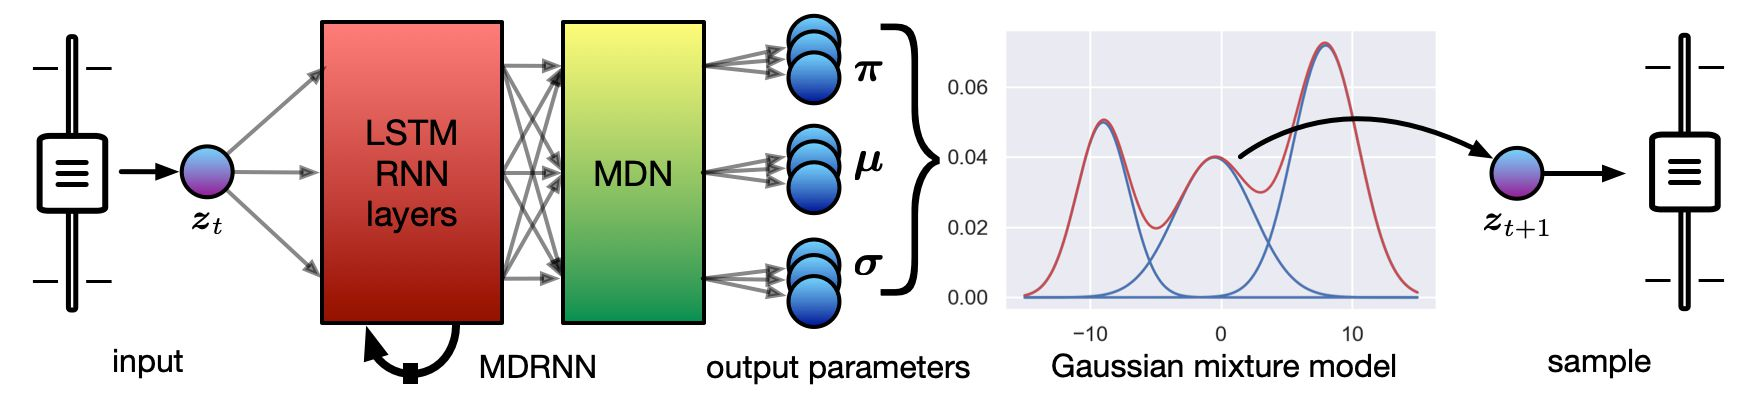
\includegraphics[width=14cm]{figures/impsy.jpg}
    \caption{Reproduction of Figure 2 from~\cite{Martin2019IMPSY} showing the IMPSY prediction process.\label{fig:IMPSY}}
\end{figure}

\subsection{Scope of our Research}
Our research aims to be a proof of concept for the use of a combined MDRNN and MCTS prediction system, and so we have limited the scope of our research to a single instrument, a monophonic 2D keyboard. While our system design is generalisable to other instruments, testing on a simple instrument allows us to focus on the core components of our system without adding unnecessary complexity. The first dimension is the required time interval dimension between control inputs, and the second dimension is pitch, which is rounded to the nearest semitone for output. Our scope is also limited to a single user, the first author of this thesis, who is a trained musician and has experience with improvisation. Ideally, a larger user study would be conducted, but was not a practical option for this project. For the evaluation of our system, we use multiple datasets to train separate models on the keyboard, and so breadth of style within the limits of a 2D monophonic keyboard is within the scope of our research. 

\section{The Prediction Algorithm}
The prediction algorithm we have developed is aimed at guiding the choice of the next control input, instead of randomly sampling it from the GMM. To do this, we create a tree of possible future control inputs over multiple predictive time steps, and choose the most promising branch of this tree to take based on a heuristic. This heuristic aims to immitate a human performers checks and balances when improvising, ensuring that intuitive musical options, which are represented by the GMM, are also musically coherent. Hence, the heuristic is based mostly on musical parameters that psychological research, as well as musical studies, have shown to be relevant the the perceptions and predictions of music by humans. The algorithm is designed to be flexible, with the exact heuristics used being customisable to the instrument used, as well as specific goals of performance or musical norms particular to a specific style or culture. All but one of the parameters used in our heuristic are generalisable to any instrument with a continuous pitch and time dimension, with the exclusion having the only additional limitation of a discrete tuning system. This is a benefit of choosing a lower dimensional instrument, and allows our heuristic configuration to act as a baseline for more specific ones to build upon. Figure~\ref{fig:Successor} shows the overall structure of our prediction algorithm, and each referenced component will be explained in more detail in the following sections.

\begin{figure}[th!]
    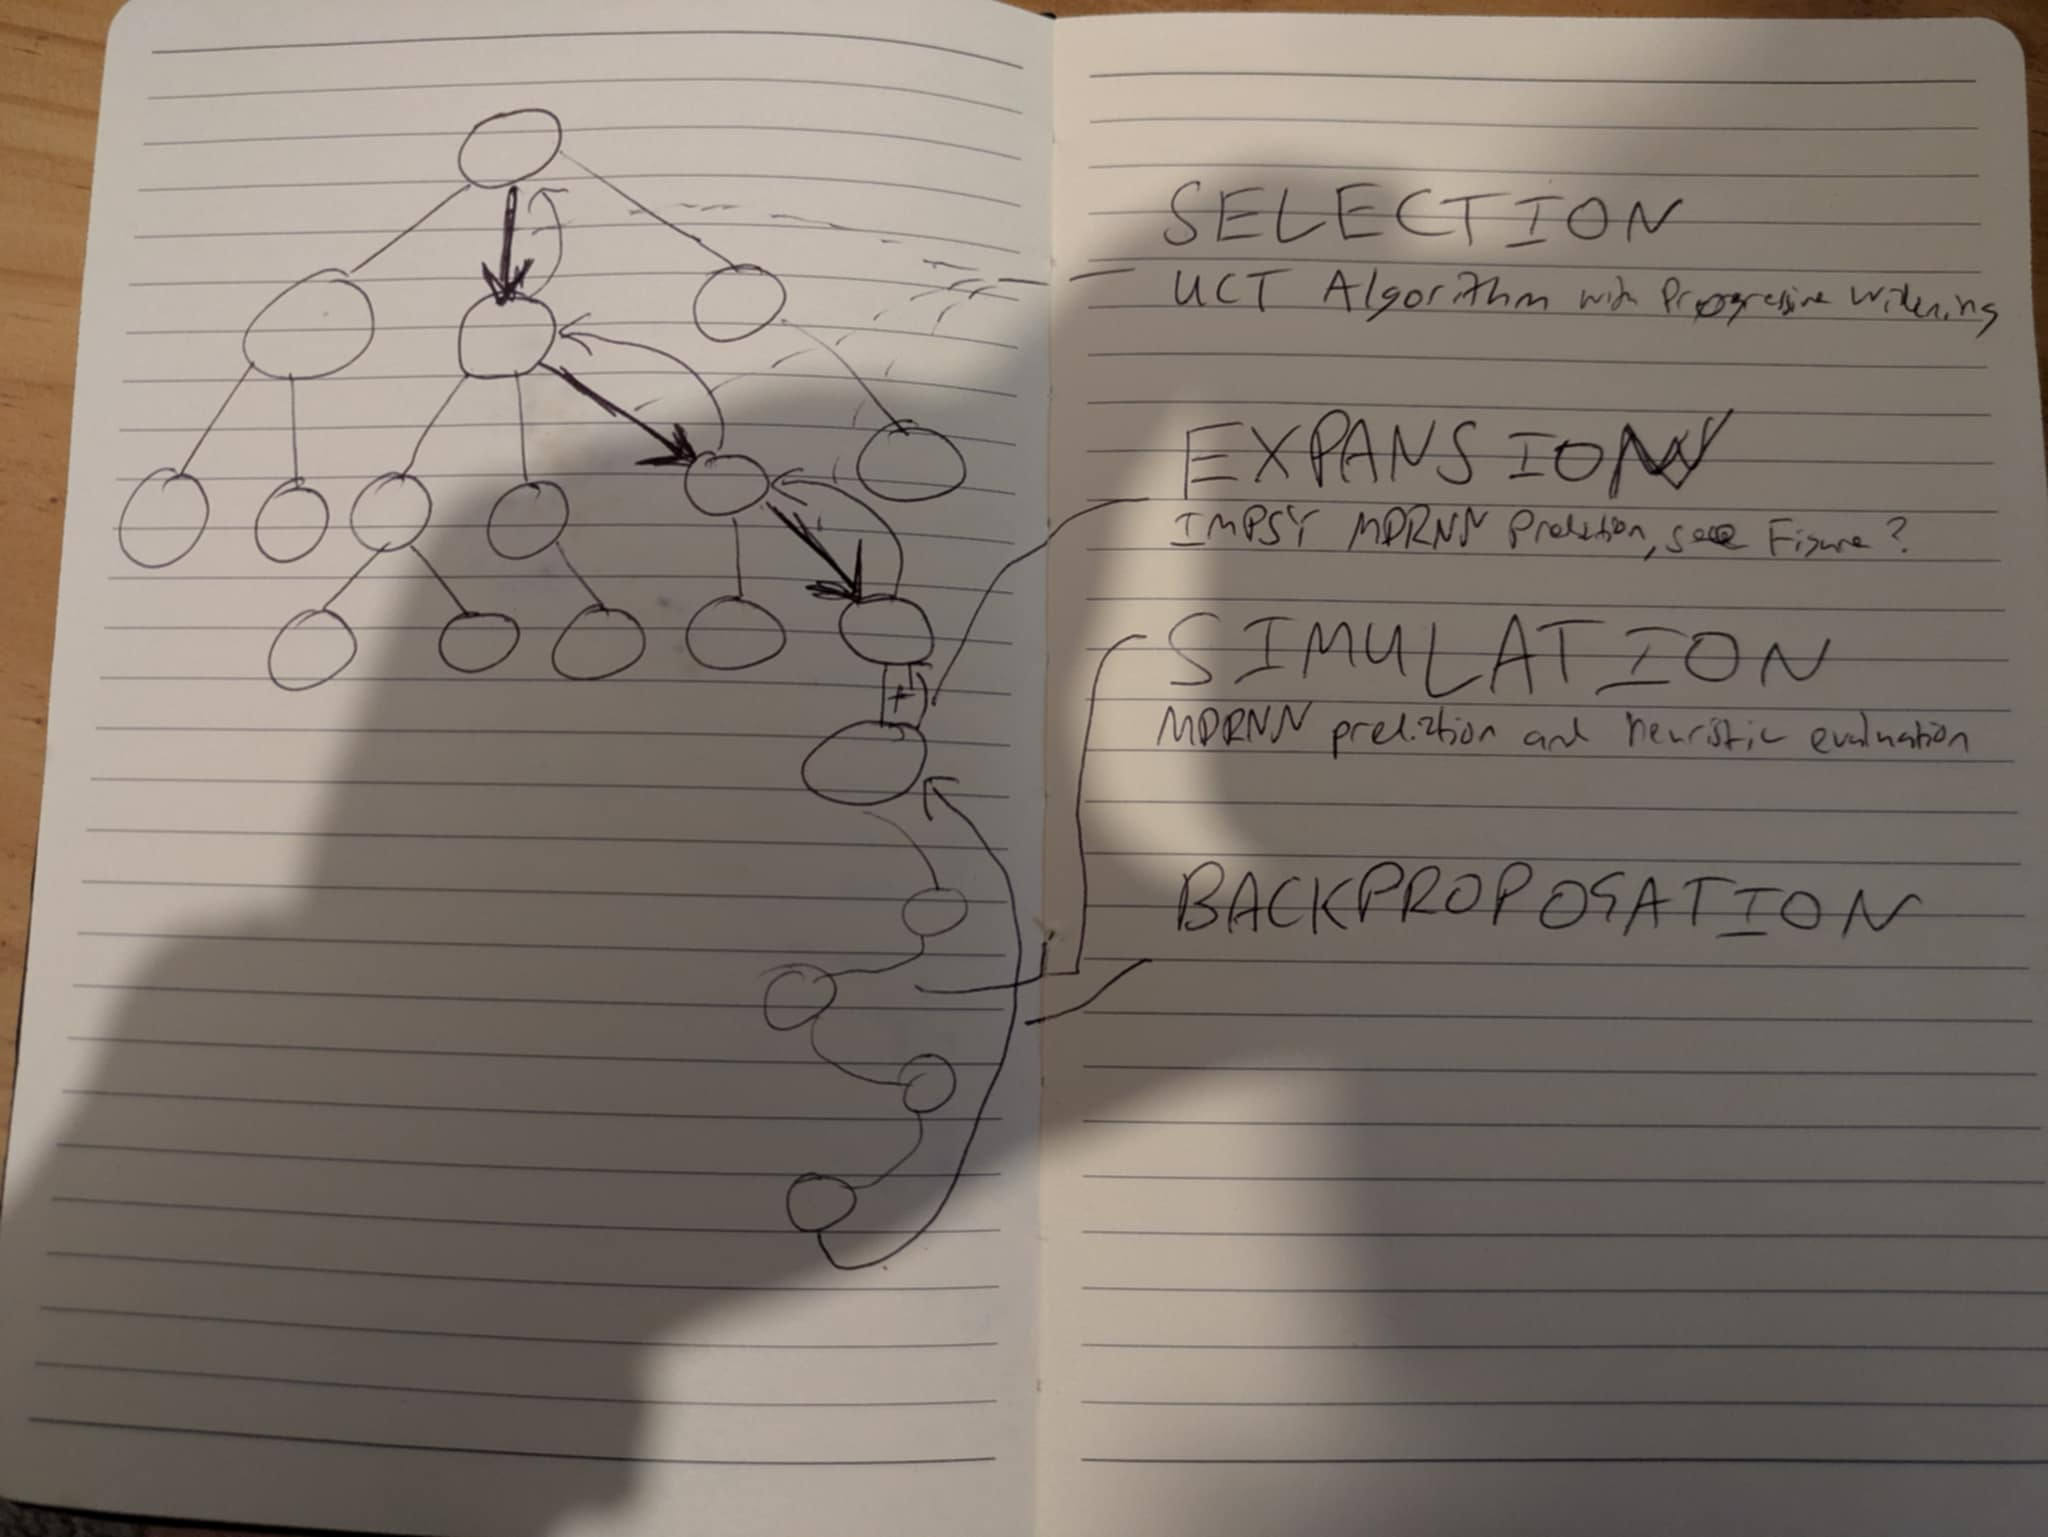
\includegraphics[width=14cm]{figures/mcts-overview.jpg}
    \caption{Our MCTS based prediction process.\label{fig:Successor}}
\end{figure}

\subsection{Monte-Carlo Tree Search}
The generate and search through a tree of predictions, the Monte Carlo Tree Search (MCTS) algorithm is used. MCTS builds a search tree incrementally and asymmetrically, focusing on the most promising parts of the search space. We start with the root node of the search, which is $z_t$, the previously output control state. From this the goal is to output a $z_{t+1}$, which will be one of the children of $z_t$ expanded in the MCTS prediction tree. Each $z_{t+1}$ is assessed by the heuristic values of its explored potential future expansions. 
The MCTS algorithm consists of looping a sequence of four main steps: selection, expansion, simulation, and backpropagation; until a set time or iteration limit for search is reached. By iterating these steps, MCTS gradually builds a search tree and improves its predictions. The algorithm's effectiveness comes from its ability to focus computational resources on the most promising parts of the search space, and at the end of search, the most visited child node of the root node is selected as the best action to take and output as $z_{t+1}$. We will now explain how each of these steps is implemented in more detail. A pseudocode version of the algorithm is shown in Algorithm~\ref{alg:CMCTS}.

\textbf{Selection:}
Starting from the root node, the algorithm selects successive child nodes until a leaf node is reached. Our selection process uses a modified version of the the Upper Confidence Bound for Trees (UCT) algorithm~\citep{Kocsis2006UCT}, which is a popular method for balancing exploration and exploitation in MCTS. The original UCT algorithm selects child nodes based on the formula:
\begin{equation}
    UCT = \frac{w_i}{n_i} + c\sqrt{\frac{\ln{N}}{n_i}}
\end{equation}
where $w_i$ is the total reward of the child node, $n_i$ is the number of visits to the child node, $N$ is the total number of visits to the parent node, and $c$ is a constant controlling the exploration-exploitation trade-off. The algorithm selects the child node with the highest UCT value. This means that it is choosing the child node with the highest average reward after simulating a potential future path. We modify UCT for our use case in two ways.

Firstly, since the action space for the children of each node is a GMM and hence continuous, we need to discretize the action space for selection. We do this by using progressive widening. Progressive widening, instead of with discrete actions where all actions are expanded at once during the expansion phase, only expands one randomly sampled action from the action space when first expanding a node. Additional nodes are added during selection if an action reaches a threshold of visits. The number of children a node $z$ has, $N_{z}$, is given by the formula:
\begin{equation}
    N_{z} = kn^{\alpha}
\end{equation}
where $n$ is the number of visits to the node, and $k$ and $\alpha$ are constants that control the growth of the action space. Whenever the calculated $N_{z_t}$ is greater than the actual number of children of $z_t$, the expansion process is triggered and a new child node is added if possible.

It is important to note the aspects of progressive widening often used in other C-MCTS implementations that are not used in our own. The most common of these are kernal regression based selection strategies such as KR-AUCB~\citep{Lei2021KBTree}. These selection strategies use modified $w_i$ and $n_i$ values to account for the fact that in a continuous action space where similar actions have similar rewards, you can have some knowledge of the reward of an action based on the rewards of its peers. $w_i$ and $n_i$ hence partially take on the values of neighbouring actions. Given that during our expansion process uniqueness for duration is heavily favoured, and pitch is necessarily substantially unique, the benefit provided by kernal regression based selection strategies is minimal and outweighed by the computational cost. It is likely that a model trained on an instrument with more continuous dimensions could reach a point where kernal regression based selection strategies would be beneficial, and so it is worth mentioning here.

Our second modification to UCT is based on the fact that UCT optimises entirely for the average reward of a child node. This is ideal for adversarial games, where another agent is fighting against you and so the average is the best you can hope for. It is also beneficial where randomness plays a large role, as an average scenario is a reasonable assumption where significant randomness is at play. However, our tree is not completely controlled by random processes, as while MDRNN sampling is random, the prediction function is not. This means that when selecting the next note at the end of search, the part of the tree under that chosen note is retained, meaning that the best found path can realistically be followed. This allows us to instead aim for paths with the maximum reward. Switching entirely to a greedy strategy would not be ideal, as it would lead to local optima and a lack of exploration. Instead, we use a modified version of the UCT algorithm which uses a weighted average of the best child node and the average child node. This is done by modifying the UCT formula to:
\begin{equation}
    UCT = \beta w_{best} + (1-\beta)\frac{w_i}{n_i} + c\sqrt{\frac{\ln{N}}{n_i}}
\end{equation}
where $w_{best}$ is the best heuristic evaluation found by the child node, and $\beta$ is a constant that controls the weighting between the best child node and the average child node, which balances greedyness in the exploitation term. This allows the algorithm to focus on the most promising future directions, while still exploring other child nodes to avoid local optima.

\textbf{Expansion:}
After reaching a leaf node, the MDRNN prediction algorithm is run to generate a GMM of possible next control inputs. This GMM is saved for the node and sampled once to generate a new child node. This child node is then added to the tree and is the starting point for the simulation process. The generated GMM will be reused for further expansion whenever progressive widening is triggered during the selection process.

During progressive widening, $c$ candidate actions are randomly sampled from the GMM. Each of these candidates are checked to ensure a distance of at least $\epsilon$ away from all existing child actions. As each dimension in the action space represents a different control parameter, different $\epsilon$ values are applied to each dimension, and a candidate action must be unique in at least one of them.$\epsilon$ also doesn't have to function as a linear distance metric, multiplicative distances and other equations can also be used. If at least one such unique action is found, then the most unique is added, where uniqueness is the sum across all dimensions of $\epsilon$ for the closest existing node, with a scaling factor applied to each dimension to account for different scales of uniqueness. If no candidate action is found the be unique progressive widening fails and no new child node is added. This is done to ensure that the search tree does not grow without reasonable exploratory potential. If progressive widening is attempted and failed 5 times in a row, it is presumed that all potential actions with any reasonable likelihood of occuring have already been added to the search tree, and so progressive widening will be disabled for this node for the remainder of the search. Figure~\ref{fig:ProgressiveWidening} visually explains the progressive widening process.

\begin{figure}[th!]
    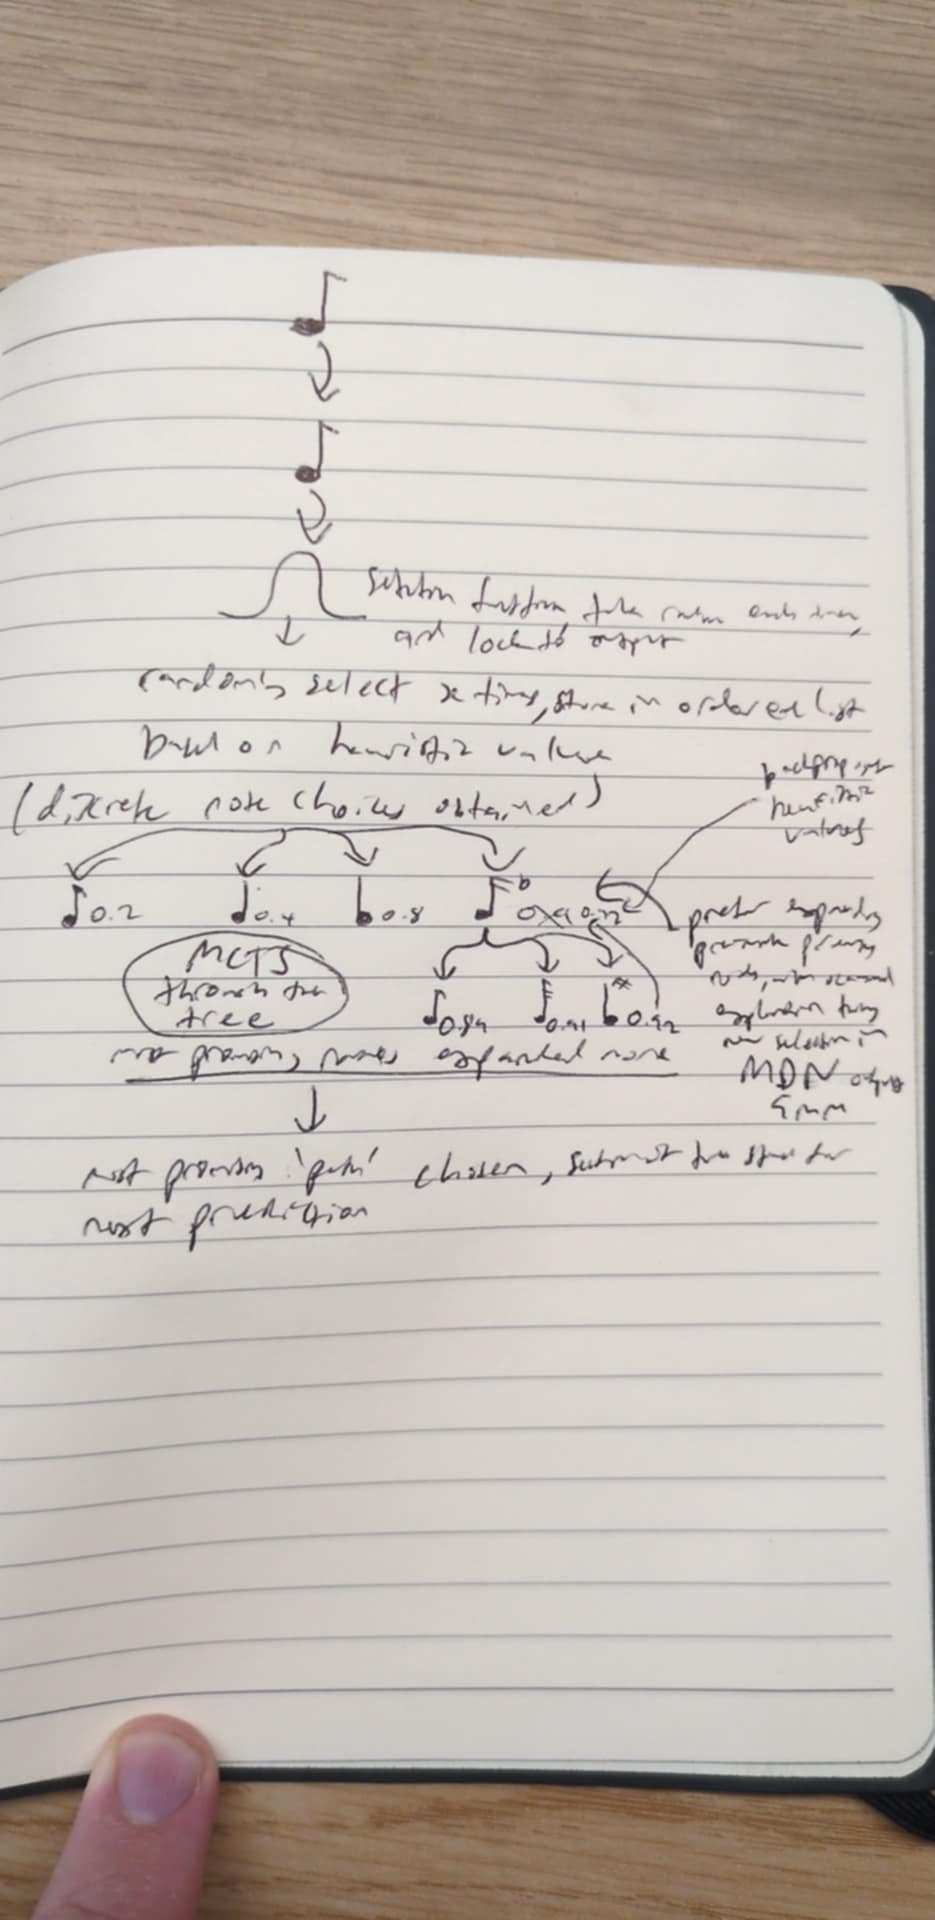
\includegraphics[width=9cm]{figures/MCTS-figure-draft.jpg}
    \caption{TODO: make this specifically a figure explaining progressive widening. C-MCTS algorithm applied to IMPSY.\label{fig:ProgressiveWidening}}
\end{figure}

Another component of progressive widening used for expansion in the literature is baysian optimisation~\citep{Mern2021BayesianMCTS}. Baysian optimisation aims to account for three key factors when expanding the action space. Firstly, which part of the action space is the most likely to be optimal based on previous searches around the area, secondly which part of the action space is the most uncertain, and thirdly how unique the candidate action is from pre-existing ones. Our method accounts for uniqueness, but does not account for uncertainty or optimality. This is because in our model nodes which were regularly visted would soon begin to fail progressive widening, meaning that no more unique actions could be added which the MDRNN gives a reasonable likelihood. This means that the entire action space is explored except for actions which is extremely unlikely or not unique enough, and hence all optimal and uncertain areas are explored without the need for a computationally expensive baysian optimisation process. As with kernal regression based selection strategies, it is likely that a model trained on an instrument with more continuous dimensions could reach a point where baysian optimisation would be beneficial, but this is not the case for our model.

\textbf{Simulation:} 
Typically in MCTS a simulation takes place from an expanded node all the way to a terminal state using some default expansion option, and the result of that terminal state is then backpropogated. However, musical prediction and improvisation does not have a terminal state, and IMPSY will continue predicting indefinitely until the user manually exits the program. Hence, a set simulation depth constant $S_d$ is used to ensure the simulation ends, and a heuristic is then run on the final state of the simulation to be used as a value for backpropogation. The simulation expansion strategy is to use default IMPSY predictions, with repeated MDRNN predictions with a random GMM sample until the simulation depth is reached. This is a computationally expensive simulation process, and so the optimal additional simulation depth after expansion was found after testing to be only 2 for search times of 100ms. This is unsurprising given the low number of iterations that can be performed within this time and the relatively expensive cost of additional simulation depth.

\textbf{Backpropagation:}
After the heuristic is run, the result is backpropogated through the tree beginning from the expanded node. The backpropagation process updates the visit count and value of each node in the path from the expanded node to the root node, as well as updating the new best heuristic value for the node if the new heuristic value is better than the previous best. These updated values are then used in the selection process, including to determine whether progressive widening should be triggered.

\begin{algorithm}
    \caption{C-MCTS Prediction Algorithm}
    \label{alg:CMCTS}
    \SetAlgoLined
    \DontPrintSemicolon
    
    \SetKwFunction{FMCTSSearch}{MCTSSearch}
    \SetKwFunction{FSelectAndExpand}{SelectAndExpand}
    \SetKwFunction{FSimulate}{Simulate}
    \SetKwFunction{FBackpropagate}{Backpropagate}
    
    \SetKwProg{Fn}{Function}{:}{}
    
    \Fn{\FMCTSSearch{memory, heuristicFunction, timeLimit}}{
        endTime $\gets$ currentTime + timeLimit\;
        \While{currentTime $<$ endTime}{
            selectedNode $\gets$ \FSelectAndExpand{root}\;
            simulationResult $\gets$ \FSimulate{selectedNode, memory, heuristicFunction}\;
            \FBackpropagate{selectedNode, simulationResult}\;
        }
        \Return{mostVisitedChild(root)}\;
    }
    
    \Fn{\FSelectAndExpand{node}}{
        \tcc{Select the best child node using UCT, widening the action space where necessary}
        current $\gets$ node\;
        \While{current.children is not empty}{
            ApplyProgressiveWidening(current)\;
            current $\gets$ UCTSelectBestChild(current)\;
        }
        \tcc{Expand final selected node}
        current $\gets$ ApplyProgressiveWidening(current)\;
        \Return{current}\;
    }
    
    \Fn{\FSimulate{node, memory, heuristicFunction}}{
        current $\gets$ node\;
        \For{$i \gets 1$ \KwTo simulationDepth}{
            current $\gets$ SampleFromGMM(current.gmm)\;
            current.gmm $\gets$ PredictWithMDRNN(current)\;
        }
        \Return{heuristicFunction(Concatenate(memory, ExtractBranch(current)))}\;
    }
    
    \Fn{\FBackpropagate{node, result}}{
        current $\gets$ node\;
        \While{current is not null}{
            current.visits $\gets$ current.visits + 1\;
            current.value $\gets$ current.value + result\;
            current $\gets$ current.parent\;
        }
    }
\end{algorithm}

\section{Heuristic Design}
For the C-MCTS algorithm to be useful, it must be guided by heuristics which detect beneficial musical branches. The heuristic in this system is based on a set of structural parameters which are measured as the user plays, and that the heuristic then attempts to emulate. To do this, our heuristic takes in the parameter values at the end of human play, and also measures the parameter values for the simulated branch of the search tree, returning the sum of the differences between these, and then inverting them, as our system maximises heuristic values and high levels of difference in parameters is unideal. Each of these parameters is based on psychological and musical research which has found these elements of composition to be parameters by which humans ourselves either intuitively or through musical learning understand musical structure and coherence and predict the future direction of music. They provide a representation for the current state of the piece a user is performing, providing a goal to which the system can aim to replicate. By guiding the musical prediction process toward outputs that humans have been shown to predict as more likely, we hypothesise that the predictive accuracy of the system can be improved. Given that the human ability to predict music is one of the core aspects of its enjoyability~\citep{Huron2008PsychOfExpectation}, we also hypothesise that this will maintain musically pleasant results which do not limit creativity and variation.

By virtue of our choice of test instrument, all but one of the parameters described here are generalisable to any instrument with a continuous pitch and time dimension. The exception is the key and modal conformity parameter, which is specific to 12TET instruments. This is added as an example of how a parameter can be added into the system to fine tune it to a specific instrument. Hypothetically, parameters could also be added to fine tune prediction toward particular styles or cultural musical norms as well, and we include examples of these in the next section.

To visually explain the relevance of this heuristic guidance, we have generated examples of how the C-MCTS algorithm can be guided. Firstly, Figure~\ref{fig:MCTSunguided} displays a tree searched with a null heuristic. This showcases potential musical directions that IMPSY would explore without our modified prediction system. Over multiple notes this becomes a wide breadth of paths due to the randomness inherent within IMPSY's predictions. As this example shows, at the particular place in the piece where the prediction algorithm has been run, a long note has been played, and the system seems to consider two reasonable future directions, continuing briefly to play longer notes before moving to shorter notes, and returning immidiately to shorter notes. Hence, despite the multitude of potential paths explored, all of them lead to shorter notes within six note predictions. In Figure~\ref{fig:MCTSguided}, we show the same C-MCTS prediction, but now using a very basic heuristic to guide the search, which favours the lowest standard deviation of time interval from the root node. This heuristic is not particularly useful in a practical sense, but provides a stark visual difference within the search tree, which is helpful for visualising the power of directed search. When guided toward paths which maintain a similar long note duration to the root note, the entire search tree shifts towards options which continue along this path. In Figure~\ref{fig:MCTSguidedpath}, we show the most visited path of the search tree from Figure~\ref{fig:MCTSguided}. This is the path that would have been taken given the heuristic guidance, and, while remaining in the realms of potential musical directions in early depths, eventually significantly diverges in musical path from the unguided search tree. These redirections of musical path which remain subtle and entirely plausible note by note, but over a longer time period adhere to heuristic guidance, is at the core of what we are trying to achieve with this system. By guiding the search tree toward plausible musical paths, we can ensure that the system is able to maintain a coherent musical direction while still allowing for the creativity and variation afforded by MDRNN predictions.

\begin{figure}[th!]
    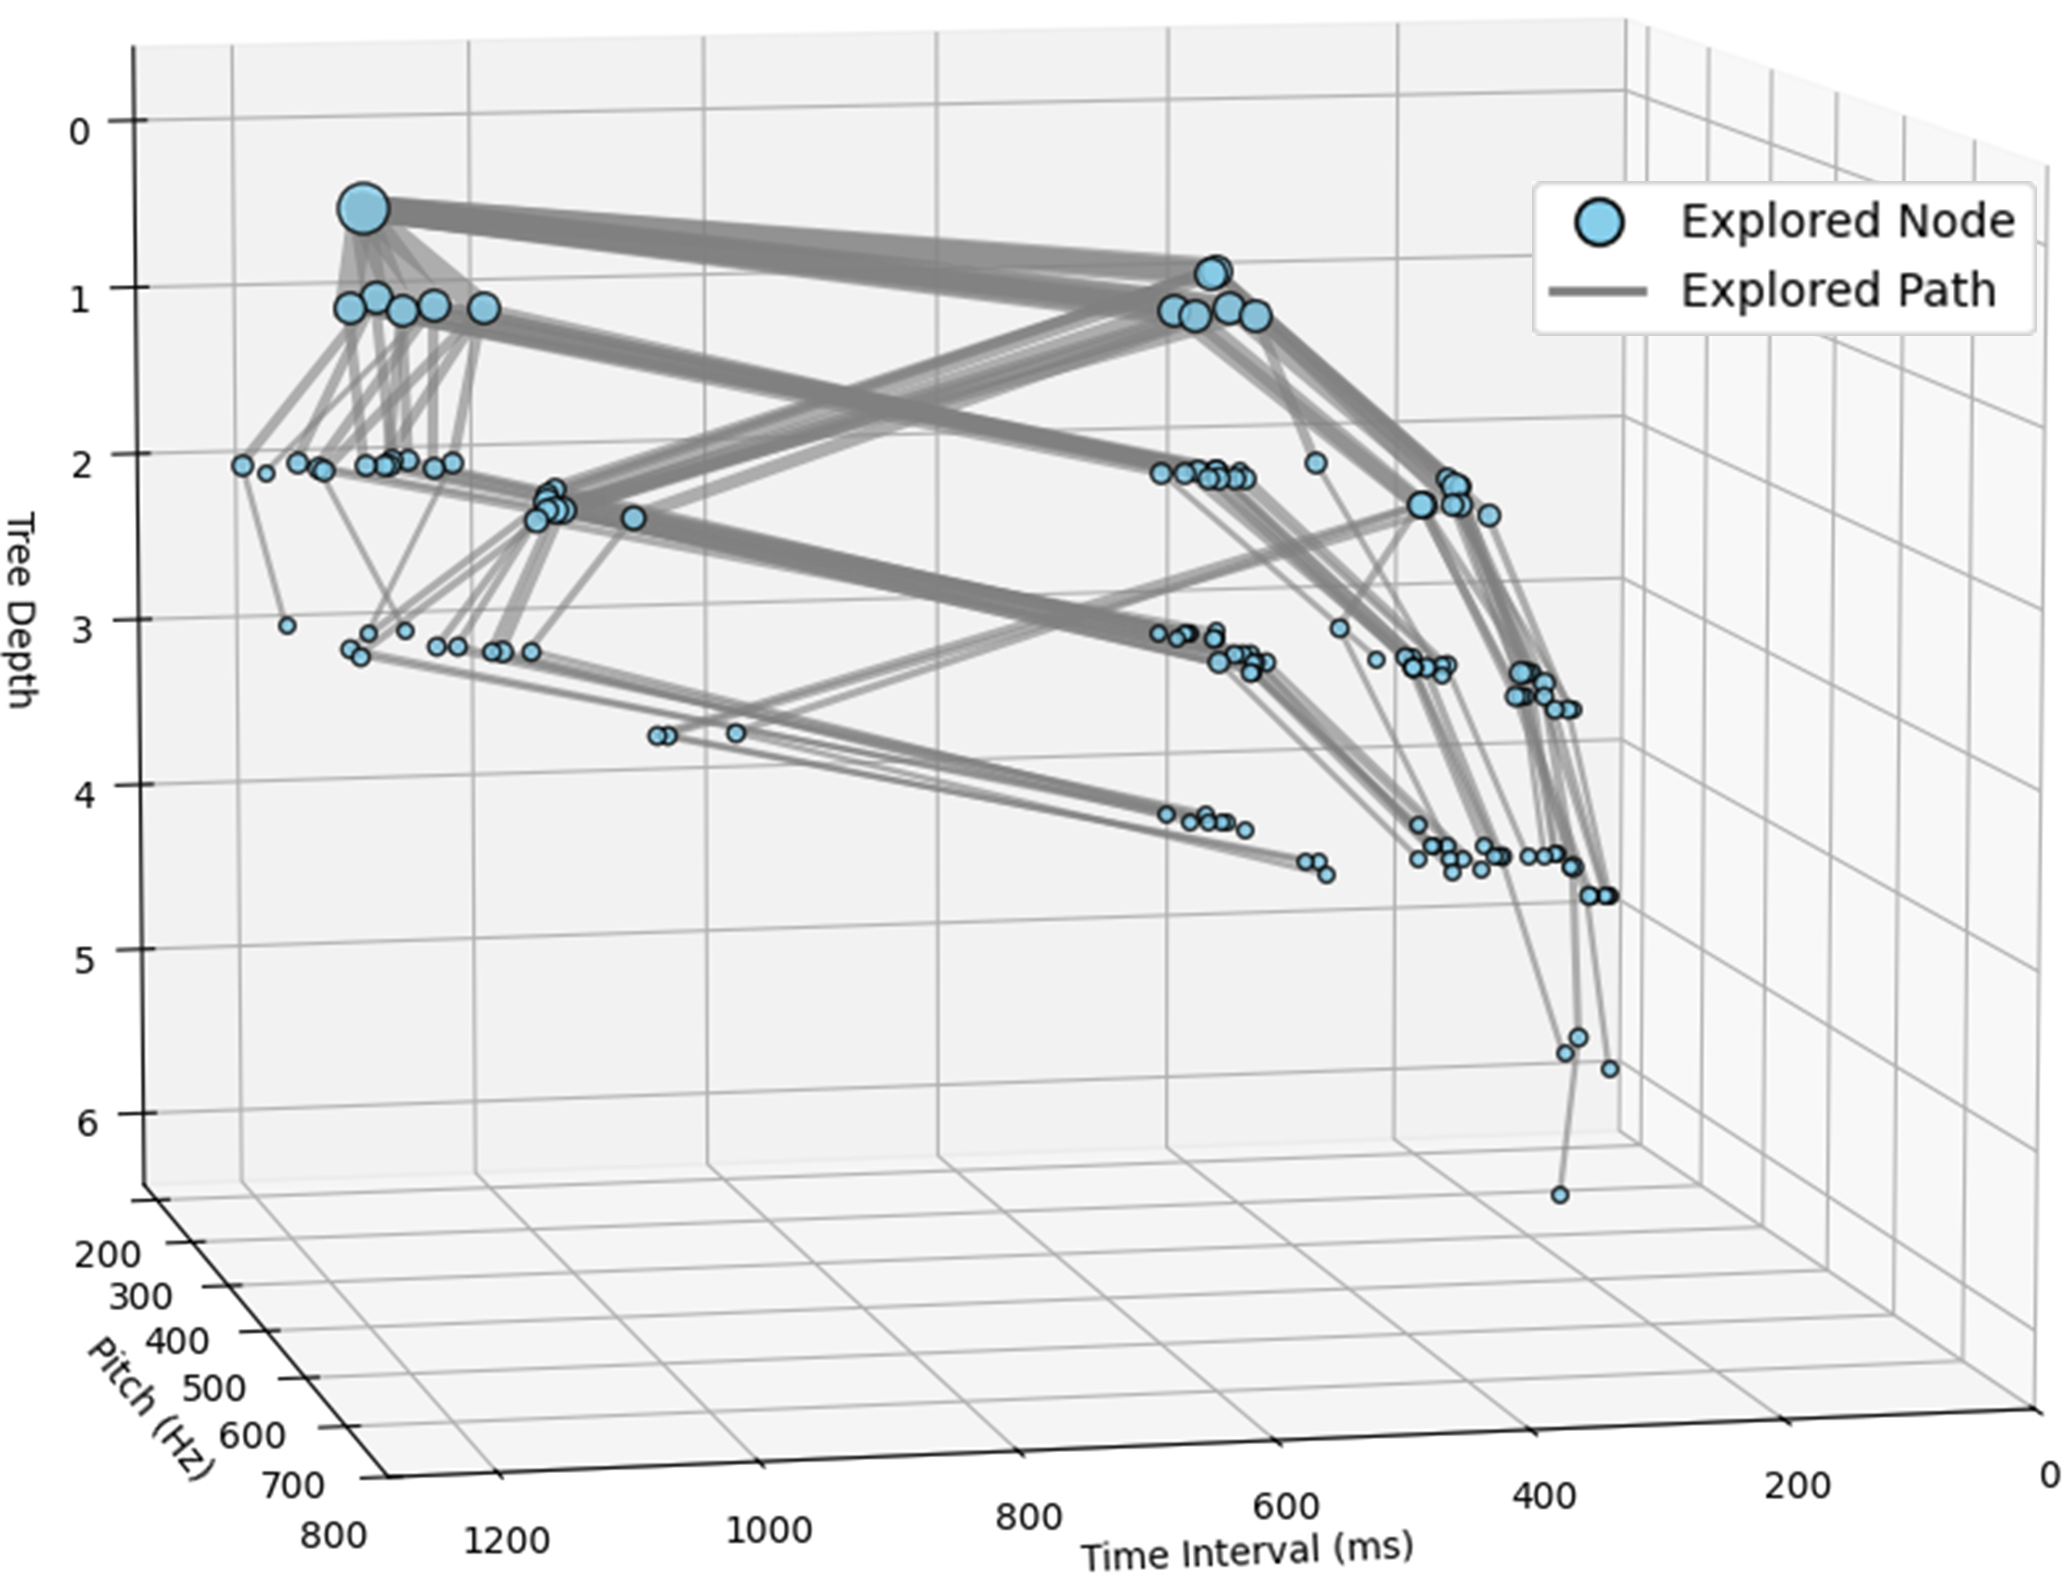
\includegraphics[width=11.1cm]{figures/mcts-unguided.png}
    \caption{C-MCTS algorithm with a null heuristic. Nodes with $\geq3$ visits are shown, with logarithmic size based on visit count.\label{fig:MCTSunguided}}
\end{figure}

\begin{figure}[th!]
    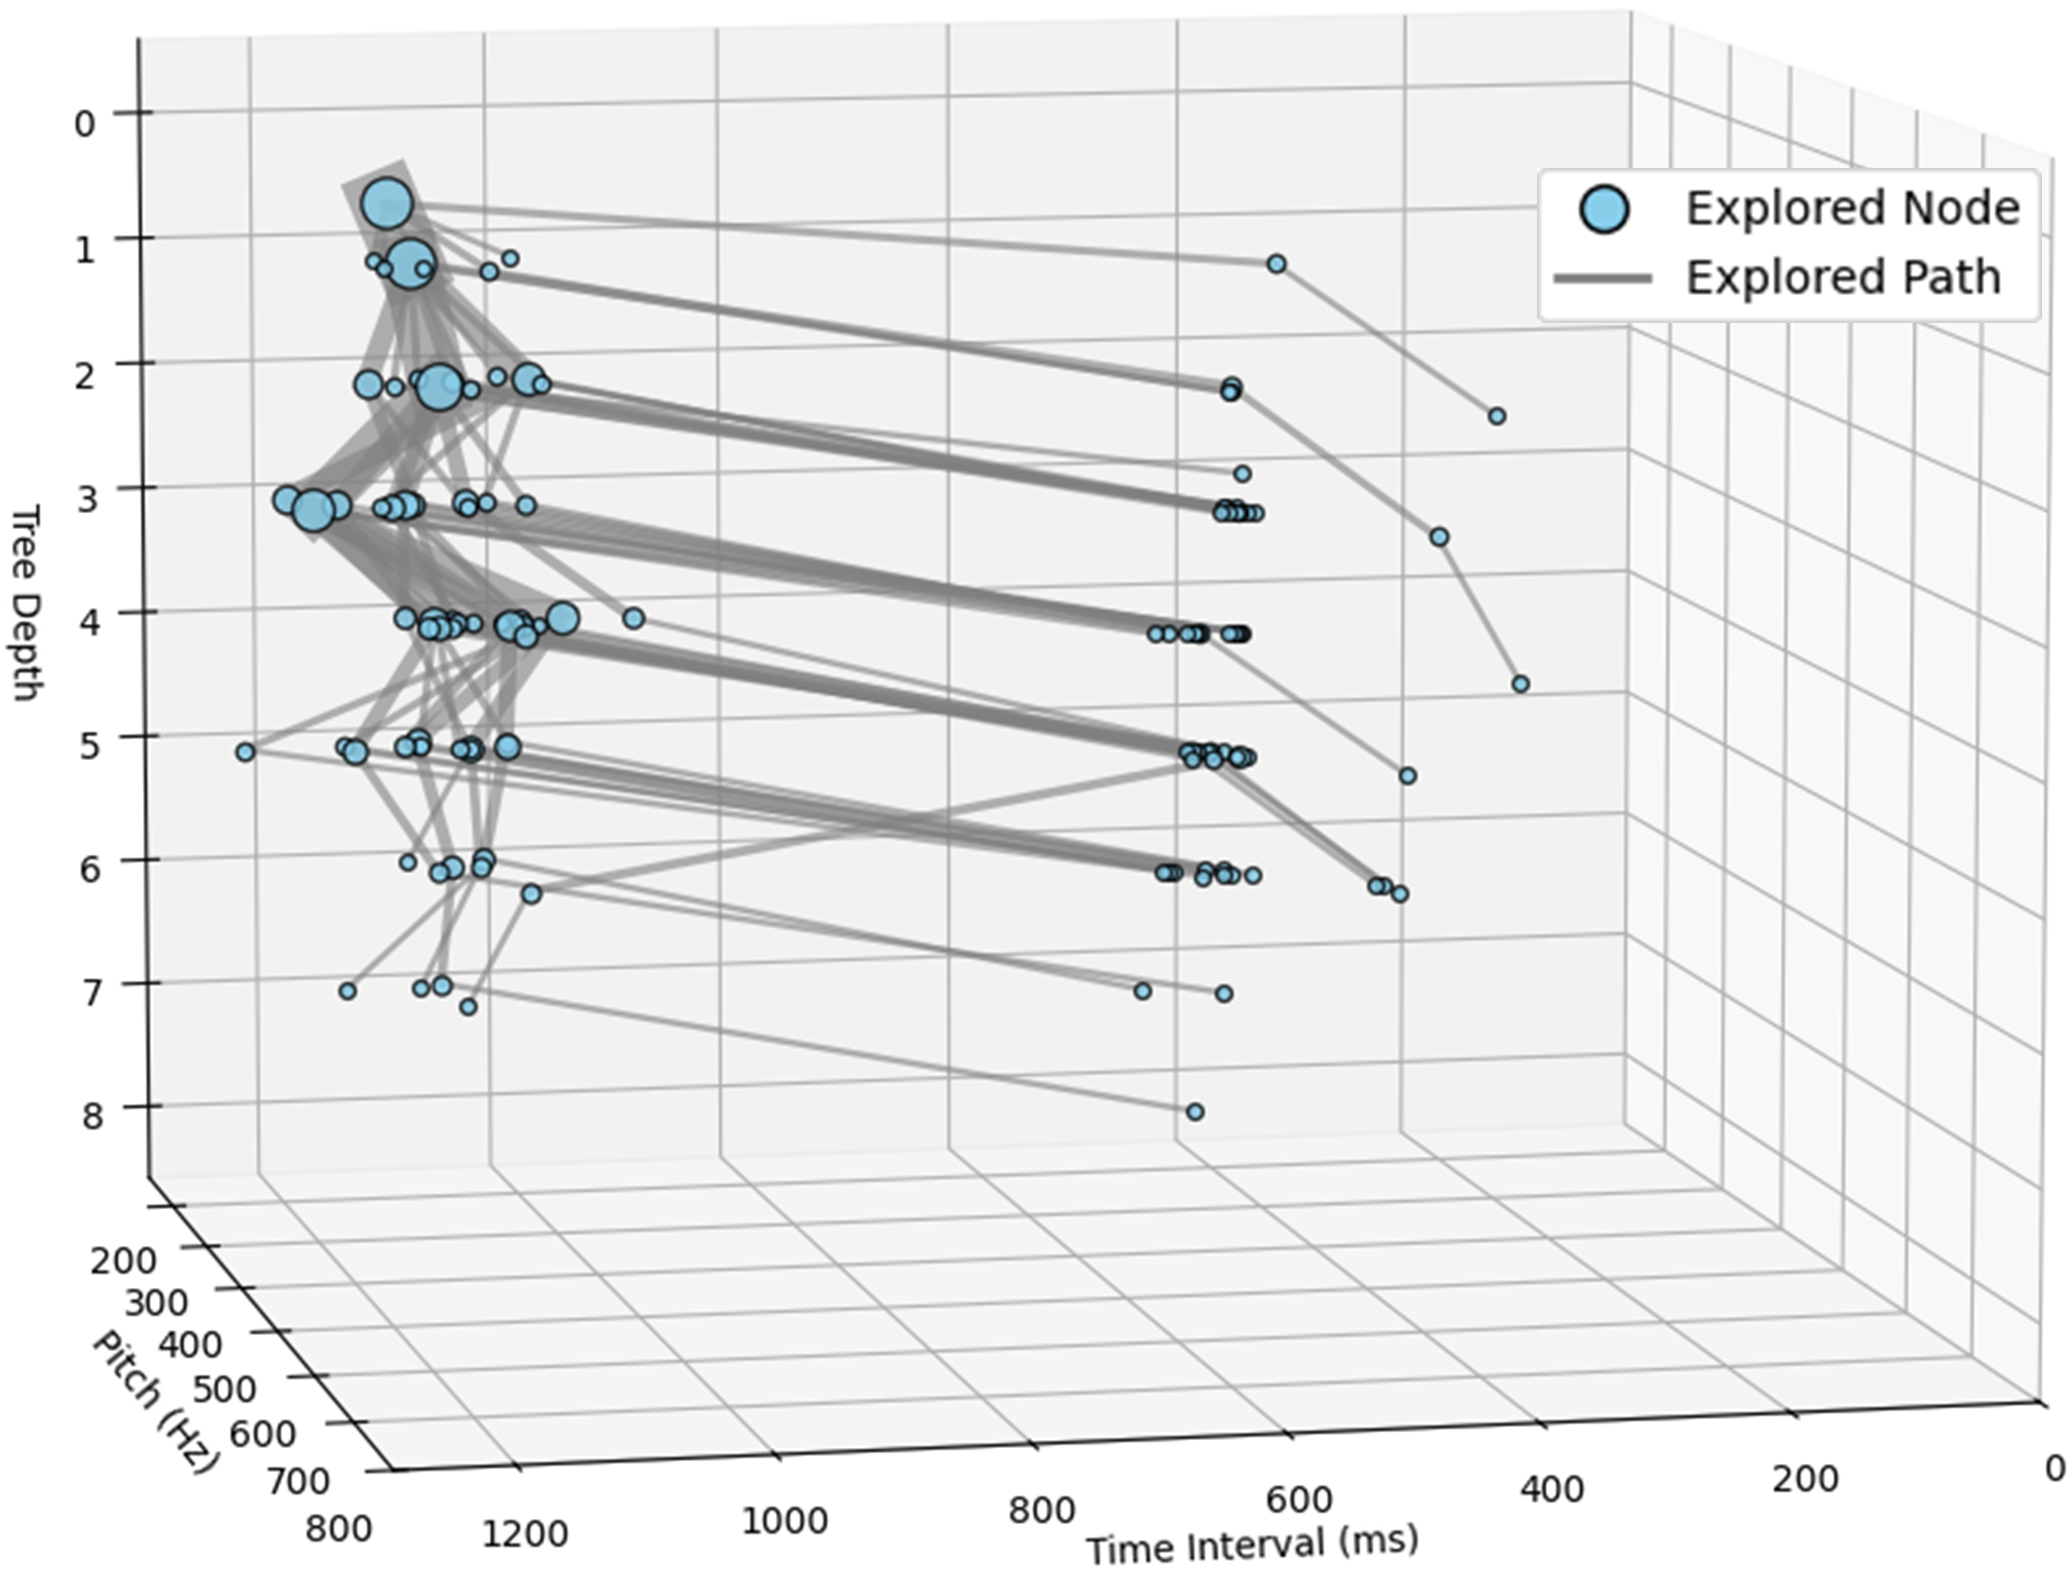
\includegraphics[width=11.1cm]{figures/mcts-guided.png}
    \caption{The same C-MCTS prediction as Figure~\ref{fig:MCTSunguided}, but with a heuristic favouring the lowest standard deviation of time interval from the root node.\label{fig:MCTSguided}}
\end{figure}

\begin{figure}[th!]
    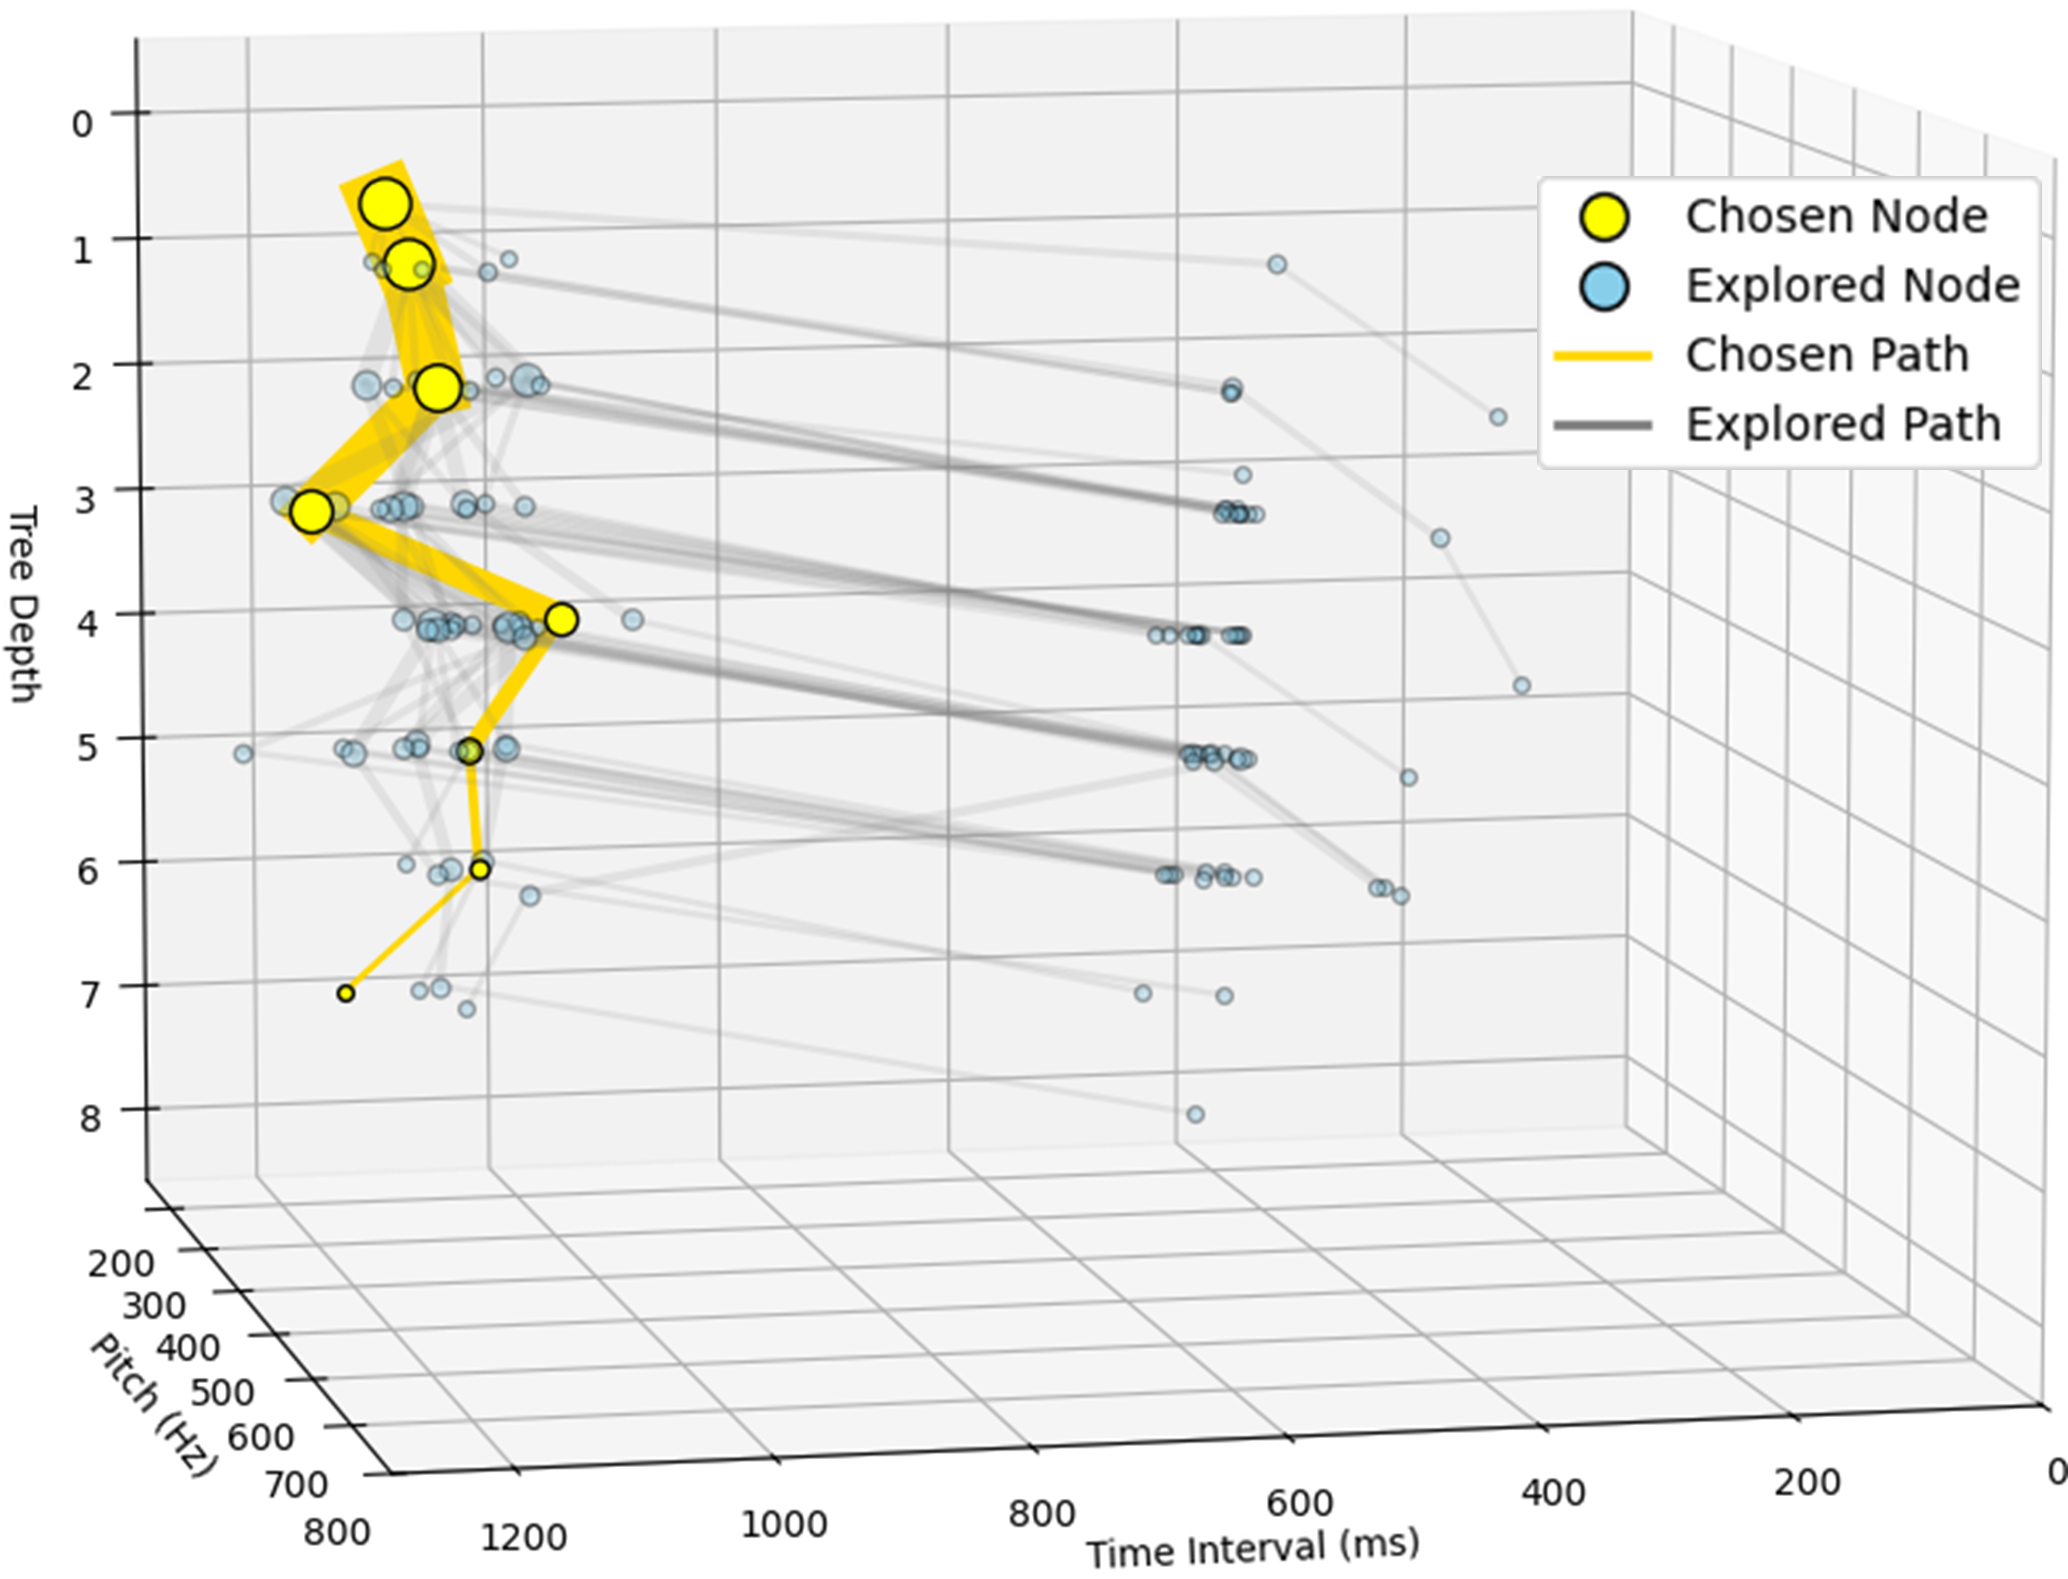
\includegraphics[width=11.1cm]{figures/mcts-guided-path.png}
    \caption{The guided C-MCTS search from Figure~\ref{fig:MCTSguided} with the most visited path highlighted.\label{fig:MCTSguidedpath}}
\end{figure}

Each of the following subsections details one of the musical parameters used in our heuristic, along with a brief justification for its importance and a description of its implementation. All of the output values of these parameters are normalised to typically remain in a range of 0 to 1, and are later given multipliers based on how well they perform for a particular model. The $n$ last human notes played, referred to as the output memory, is kept and used to determine current parameter values to aim toward.

\subsection{Key and Modal Conformity}

Key and modal conformity measures how well musical branches adhere to the established musical scale and mode in the output memory, if such a scale and mode clearly exists.~\cite{Temperley2008MelodyPerception} explores this through the concept of a key profile, noting that keys and modes are key factors in human prediction of the likelihood of musical continuations, particularly in Western music. The key profiles model is based on two observations about melodies which conform to a particular key. Firstly that notes within that key are significantly more likely to be used than those outside of it, and secondly that notes of the tonic triad, the root, third, and fifth of the scale, are slightly more likely to be used than other notes within the key. However, the likelihoods of each note are combined into a single key profile in this paper, which only accounts for natural major and minor scales, showing the increased use of the sharp sixth and seventh degrees in minor scales as small increases in usage within a natural minor key profile, instead of recognising the distinction of melodic and harmonic minor scales, and completely ignoring the use of other modes and key types.

To address these limitations we modify the key profiles methodology from the above paper into two parameters, a key conformity and modal conformity parameter, which combine as one of the five individual parameter heuristics combined into the final heuristic for our system. Key conformity doesn't account for a root note, and instead only looks at the relative use of notes within a given scale. Because of this it is a lot easier to include more varieties of scale, and our parameter tests against four common scale types: major, pentatonic, blues, and harmonic minor; although it is trivial to add more if relevant to a particular style. For each scale type, the algorithm considers all possible transpositions (root notes) and calculates a conformity value for the output memory using the formula: 
\[\text{key conformity} = \frac{12k - n}{12 - n}\]
Where $k$ is the proportion of notes in the output memory which belong to the scale and $n$ is the number of notes in the scale being tested. This formula normalizes the conformity measurement across scales with different numbers of notes, yielding values between -1 (complete non-conformity) and 1 (complete conformity), with a value of 0 being expected for a random sequence of notes. The system selects the scale type and root note combination that produces the highest conformity value, provided it exceeds a minimum threshold constant which through testing has been set at 0.7. If no scale exceeds this threshold, the system does not use key or modal conformity for that prediction tree.

The modal conformity parameter extends the key conformity parameter when a valid key match is found by determining which mode within the identified scale is being emphasized. This allows every potential mode of any scale to be checked, as opposed to only major or minor. For each potential mode the system establishes which notes are within the root triad and then calculates a mode conformity value for the output memory using the formula:
\[\text{mode conformity} = \frac{nk_t - 3}{n - 3}\]
Where $k_t$ is the proportion of scale-conforming notes that also belong to the identified triad and $n$ is the number of notes in the scale. This once again normalizes the conformity measurement across scales with different numbers of notes and yields values between -1 and 1. The system selects the mode with the highest conformity value, provided it exceeds a minimum threshold constant which through testing has been set at 0.25. If no mode exceeds this threshold, the system does not use modal conformity for that prediction tree, only key conformity.

These initial calculations are performed for the output memory when the system first takes over performance and a new MCTS tree instance is created. Hence, when evaluating potential branches in the search tree, key and mode conformity values only need to be calculated against the established key and mode of the output memory, if such a key and mode was determined to exist. The returned heuristic value is calculated as:
\[\text{heuristic} = \left(|b_k - m_k| + \min\left(\frac{|b_m - m_m|}{d_m}, l_m\right)\right) \cdot \text{multiplier}\]
Where $b_k$ and $m_k$ are the branch and memory key conformity values, $b_m$ and $m_m$ are the branch and memory mode conformity values, $d_m$ is a constant representing the weight of the node conformity compared to key conformity which through testing is set to 3.0 in our model, $l_m$ is a constant limiting the effect of mode difference when a mode is completely different which we set to 0.15, and a multiplier scales the overall heuristic value compared to others included in the final heuristic calculation. This is adjusted based on model and so will be discussed in the evaluation.

This dual approach to key profiles allows the system to maintain consistency with the performer's key and mode if they are adhering to one, while not affecting results if it is not clear that they are. The algorithm also adapts to the performer's level of key adherence, preferencing occasional out of key notes if they are present in the output memory. The separation into two parameters also allows for more versitility, incorporating any desired scale in any mode. Unlike the other heuristics in the system, key and modal conformity is specific to instruments using twelve-tone equal temperament (12TET) or another tuning system with discrete notes if adapted, as the existence of keys and modes relies on this. Hence, in a loose sense this is an example of how more instrument and style specific parameters can be integrated into the system to enhance its performance for particular contexts.

TODO: analyse a figure showing a short piece of sheet music and two possible continuations, provide an example heuristic evaluation of them.

\begin{figure}[th!]
    
\includegraphics[width=11.1cm]{figures/todo.jpg}
    \caption{TODO: analyse a figure showing a short piece of sheet music and two possible continuations, provide an example heuristic evaluation of them.\label{fig:TODO}}
\end{figure}

\subsection{Tempo and Swing Conformity}

Tempo and swing conformity measures how well musical branches adhere to the established tempo and swing in the output memory, if a constant tempo and swing clearly exists. Tempo and swing are fundamental rhythmic parameters in music that play a large part in rhythmic expectation and prediction.~\cite{Laroche2001TempoEstimation} discusses this importance, and establishes a method for estimating the tempo (speed), swing (rhythmic inequality of eighth notes), and downbeat (the first and usually strongest beat of a measure) of a piece of music. This method starts from an audio track, first establishing the location of notes from the audio, before performing analysis on these note locations to establish rythmic parameters. Since our system receives note locations directly as control inputs, we skip the first step of this process. Establishing downbeats also relies on the volume of notes, which is not available in our current 2D keyboard implementation, and so only tempo and swing are used in our system, with a modified implementation.

The tempo and swing heuristic operates by examining the durations between note onsets to determine the most likely tempo in beats per minute (BPM) and the type of swing feel being employed. The system evaluates these patterns by comparing actual note durations against expected durations that would occur in various tempo and swing combinations. For any given tempo, the algorithm calculates expected note durations for common rhythmic values, from sixteenth notes up to whole notes, as well as the dotted (1.5x length) variants of these notes. For swing, the standard eighth note is replaced with two swung eighth notes, a long and short note, with a ratio determined by their level of swing. For our model only triplet swing (2:1 ratio) is used, as this is the most common type of swing in Western music, however, it is trivial to add more swing types if desired.

To determine the rhythm of the output memory, the algorithm scans across a range of tempos (default 70-138 BPM in 2 BPM increments) for both no swing and triplet swing, and calculates the average deviation score of the output memory. The deviation score for each note is calculated as:
\[\text{deviation} = \text{penalty} + \frac{|\text{actual} - \text{expected}|}{\text{expected}}\]
Where the penalty is a small additional cost applied to less likely but still possible note durations in a given tempo, such as dotted notes. The system also applies a penalty when consecutive long swing notes are detected, as this pattern typically indicates a misclassification of the rhythm rather than actual swing. A tempo conformity score is then calculated for each tempo and swing option:
\[\text{tempo conformity} = 1 - \frac{\text{average deviation score}}{\text{maximum acceptable deviation}}\]
Where the maximum acceptable deviation (default 0.08) represents the threshold beyond which a performance would be considered rhythmically inconsistent. The tempo and swing value with the maximum tempo conformity score are selected as the best fit for the output memory, provided there is at least one positive score. If no positive score is found, there is no clear static tempo, and the system does not apply this heuristic.

When evaluating potential branches in the search tree, the heuristic determines the average deviation of the branch for the established tempo and swing of the output memory. For branches with a lower average deviation than the output memory, the heuristic returns zero, allowing other heuristics to guide the search. For branches that receive a higher score, the heuristic returns the following value:
\[\text{heuristic} = \text{memory tempo conformity} \times (\text{branch average deviation} - \text{memory average deviation}) \times \text{multiplier}\]

This approach scales the relative effect of this heuristic based on the level of tempo conformity in the output memory, as well as with an additional overall scaling multiplier. It rewards branches that best maintain the established tempo and swing of the output memory where this tempo and swing is clear, and does not have an effect where it is not, hence not negatively affecting results where the performer is using variable tempo or swing.

TODO: analyse a figure showing a short piece of sheet music and two possible continuations, provide an example heuristic evaluation of them.

\begin{figure}[th!]
    
\includegraphics[width=11.1cm]{figures/todo.jpg}
    \caption{TODO: analyse a figure showing a short piece of sheet music and two possible continuations, provide an example heuristic evaluation of them.\label{fig:TODO2}}
\end{figure}

\subsection{Pitch Interval Markov Model}

The Pitch Interval Markov Model heuristic captures melodic patterns by analyzing the intervals between consecutive notes. Early experiments into melody distortion by~\citep{White1960MelodyRecognition} tested which changes to melody most affected recognition, and established the importance of melodic contour and interval size.~\citep{Dowling1971Contour} conducted more rigourous experiments on these factors in particularly, and showed that there are three levels to melody recognition. The most fundamental of these is the maintainence of contour, or the direction of pitch movement from each note to the next. One step above this is the maintainence of intervals, or the distance between each note. The final level is the maintainence of absolute pitch, or in essense repetition of the same melody. The addition of each of these factors improves melody recognition. These factors have later been used to to establish their importance in melody prediction~\citep{Temperley2008MelodyPerception}, with it seeming that memory of the direction of pitch and intervals between notes in a melody significantly influence perceived probability of melodic continuations. Hence, we aim to recreate this prediction process as a heuristic parameter in our system.

Initial testing showed that melodic contour based heuristics provided minimal effectiveness, likely due to them being relatively simple and hence likely mostly encompassed already by the neural network predictions. Hence, we instead focus on the second level of melody recognition, the maintainence of intervals. To replicate as best as possible the findings of~\citep{Temperley2008MelodyPerception}, we use a Markov model to predict the next interval based on changes in interval detected in the output memory. The heuristic is set up to allow for any n-order markov model, but a first-order model was found to be the most effective in our tests and is the version which will be described here. 

The model is contructed as follows:
\begin{itemize}
    \item Extract the sequence of pitch values from the output memory and convert them to MIDI note numbers (integers from 0-127)
    \item Calculate the intervals between consecutive notes (the difference between adjacent pitch values)
    \item For each interval, record the frequency with which each possible interval follows that interval in the output memory
    \item Represent the model as a dictionary where the keys are the intervals and the values are dictionaries mapping each possible next interval to its frequency 
\end{itemize}

For example, a key of 2 with a value mapping of \{1: 5, -4: 2\} indicates that after the melody moved up by 2 semitones in the output memory, there were five instances where it then moved up by 1 semitone and two instances where it moved down by 4 semitones.

When evaluating branches in the search tree, the branches are converted to interval sequences in the same way as the output memory. The heuristic then calculates the probability of each interval transition in the branch according to the generated markov model. This is based on the frequencies in the markov model, with Laplace smoothing applied to account for the fact that intervals not observed in th output memory should still have some probability of occuring. The formula for calculating the transition probability with smoothing is:
\[P(\text{next_interval}|\text{current_interval}) = \frac{\text{count}(\text{current_interval}, \text{next_interval}) + \alpha}{\text{count}(\text{current_interval}) + \alpha \times |\text{transitions}|}\]
Where $\text{count}(\text{current_interval}, \text{next_interval})$ is the number of times in the model that the next interval follows the current interval, $\text{count}(\text{current_interval})$ is the total number of transitions from the current interval, $|\text{transitions}|$ is the number of unique transitions observed from the current interval, and $\alpha$ is the Laplace smoothing parameter, which through testing was set to 0.1.

The system calculates the average probability across all transitions in the branch and returns the inverse value (multiplied by a scaling factor) as the heuristic score:
\[\text{heuristic} = (1 - \text{average probability}) \times \text{multiplier}\]
This formulation ensures that branches with interval patterns similar to those in the performer's playing receive lower heuristic scores (indicating better conformity), while branches containing unusual or unseen interval sequences receive higher scores.
The interval Markov model is particularly effective at capturing the characteristic "vocabulary" of melodic patterns a performer uses while allowing for creative variations within that style. By focusing on intervals rather than absolute pitches, the model generalizes across different keys and registers, making it applicable to a wide range of musical contexts and styles from simple diatonic melodies to complex chromatic passages. It is partciularly useful during sections where repeated intervalic patterns are present, such as an arpeggio.

TODO: analyse a figure showing a short piece of sheet music and two possible continuations, provide an example heuristic evaluation of them.

\begin{figure}[th!]
    
\includegraphics[width=11.1cm]{figures/todo.jpg}
    \caption{TODO: analyse a figure showing a short piece of sheet music and two possible continuations, provide an example heuristic evaluation of them.\label{fig:TODO3}}
\end{figure}

\subsection{Time Multiple Markov Model}

Rhythmic contour has been found to be at least as important as pitch contour in melody perception~\citep{Dowling1999RhythmContour}. Similar experiments to those performed by~\citep{Dowling1971Contour} for pitch contour have also be performed for rhythmic contour, and have shown very similar results~\citep{Schmuckler2023RhythmContour}. Given the similarities between these two factors, for this heuristic we use a very similar approach to the pitch interval markov model heuristic. However, there are two important differences in model construction. Firstly, the time multiple markov model uses the ratios between consecutive note durations rather than the difference between them. This is because it is relative proportions which determine rhythmic patterns and equate to the role of intervals in pitch. Technically, for pitch intervals ratios were also used, however since frequency values are converted to MIDI notes numbers, multiplicative distances are converted to additive distances. The second difference is that time operates on a continuous scale in our model, whereas pitch operates on a discrete scale. Hence for a markov model to work, multiples between pitches must first be quantized to a discrete scale. These time multiples are quantized to the multiplicatively closest value in the set $\text{Valid multiples} = {0.125, 0.25, 0.33, 0.5, 0.67, 1.0, 1.5, 2.0, 3.0, 4.0, 8.0}$, with a small distance penalty for multiples outside of the set $\text{Common multiples} = {0.25, 0.5, 1.0, 2.0, 4.0}$.

The model is contructed as follows:
\begin{itemize}
    \item Extract the sequence of time intervals from the output memory
    \item Calculate the multiple between consecutive time intervals (eg 1.2 seconds to 0.3 seconds would be 0.25)
    \item Quantize the multiples to the nearest value in the set of valid multiples, with a small distance penalty for less common multiples
    \item For each quantized multiple, record the frequency with which each other quantized multiple follows that interval in the output memory
    \item Represent the model as a dictionary where the keys are the quantized multiples and the values are dictionaries mapping each possible next quantized multiple to its frequency 
\end{itemize}
For example, a key of 0.25 with a value mapping of \{4: 3, 3: 1\} indicates that after a given note had a quarter of the duration of its predecessor, there were three instances where the next note had four times the duration of that given note, and one instance where the next note had three times the duration.

Once this markov model is constructed, the process to evaluate branches is the same as for the pitch interval markov model. The transition probabilities are calculated using the same laplace smoothing constant of $\alpha = 0.1$, using the formula:
\[P(\text{next_multiple}|\text{current_multiple}) = \frac{\text{count}(\text{current_multiple}, \text{next_multiple}) + \alpha}{\text{count}(\text{current_multiple}) + \alpha \times |\text{transitions}|}\]
The system then calculates the average probability across all transitions in the branch and returns a scaled inverse as the heuristic score:
\[\text{heuristic} = (1 - \text{average probability}) \times \text{multiplier}\]
The Time Multiple Markov Model is particularly effective at capturing rhythmic patterns, and can do so even when there is no strict tempo sue to the note by note way that quanitzation is done.

TODO: analyse a figure showing a short piece of sheet music and two possible continuations, provide an example heuristic evaluation of them.

\begin{figure}[th!]
    
\includegraphics[width=11.1cm]{figures/todo.jpg}
    \caption{TODO: analyse a figure showing a short piece of sheet music and two possible continuations, provide an example heuristic evaluation of them.\label{fig:TODO4}}
\end{figure}

\subsection{Repetition Markov Model}

The Repetition Markov Model heuristic identifies repetition by combining pitch intervals and time multiples from the previous two heuristics into a single second-order markov model.~\citep{Duane2016Repetition} shows that identifying repetition plays a key role in musical prediction probabilities, but also that to maintain originality and prominent sections within a piece, this repetition must be balanced with variation. To create this balance, strict rules are placed on when the repetition model comes into effect. No Laplace smoothing is applied, and the second-order model ensures that this heuristic will only influence the search tree when a clear motif is established through multiple note transitions in a row which are repeated. The maintainence of relative instead of absolute measures of pitch and time also allows for transposed motifs to be recognised, which is important for the system to be able to change keys and perform well in different octaves.

The model is contructed as follows:
\begin{itemize}
    \item Extract the sequence of pitch values and time intervals from the output memory, converting pitches to MIDI note numbers
    \item Calculate the pitch intervals and quantized time multiples between consecutive notes
    \item For each tuple of (pitch\_interval, time\_multiple), record the frequency with which each possible next tuple follows that tuple in the output memory
    \item Represent the model as a nested dictionary where:
    \begin{itemize}
        \item The keys of the outer dictionary represent a state, which is a tuple of two consecutive paired environments
        \item The keys of the inner dictionaries are each individual paired event which follows that state in the output memory
        \item The values of the inner dictionaries are frequency counts for this continuation
    \end{itemize}
\end{itemize}
For example, a key of ((2, 1.0), (-3, 0.5)) with a value mapping of \{(1, 2.0): 3\} indicates that after an upward step of 2 semitones with equal duration followed by a downward movement of 3 semitones at half the previous duration, the next event was always an upward step of 1 semitone with twice the previous duration, and this specific pattern occurred three times in the output memory.

Unlike the other Markov models, the Repetition Markov Model does not apply Laplace smoothing to unseen transitions. Instead, it assigns a probability of zero to any state-transition pair that was not observed in the performer's playing. This design choice deliberately emphasizes exact repetition of musical motifs, and leads to the following transition probability calculation:
\[P(\text{next note}|\text{state}) = \begin{cases}
\frac{\text{count}(\text{state}, \text{next note})}{\text{count}(\text{state})}, \& \text{if the transition was observed} \
0, \& \text{otherwise}
\end{cases}\]
The system calculates the average probability across all transitions in the branch and returns a scaled inverse as the heuristic score:
$\text{heuristic} = (1 - \text{average probability}) \times \text{multiplier}$
This formulation ensures that branches containing exact repetitions of motifs from the performer's playing receive lower heuristic scores (indicating better conformity), while branches with novel combinations receive higher scores. However, in instances where the performer has not established a clear motif, this heuristic will not influence the search tree, allowing other heuristics to guide the search. This encourages the continuation of established motifs and thematic material to reinforce the structural coherence of the performance, but limits its potential negative impact on the originality of the generated music.

TODO: analyse a figure showing a short piece of sheet music and two possible continuations, provide an example heuristic evaluation of them.

\begin{figure}[th!]
    
\includegraphics[width=11.1cm]{figures/todo.jpg}
    \caption{TODO: analyse a figure showing a short piece of sheet music and two possible continuations, provide an example heuristic evaluation of them.\label{fig:TODO5}}
\end{figure}

\subsection{Failed Parameters}
Pitch range, height and proximity
TODO: Inlcude in later section, analyse why this doesn't work, too simple of patterns, definitely already covered by the MDRNN prediction, and hence adding extra more simple restrictions only limits the MDRNN instead of improving it.
~\citep{Temperley2008MelodyPerception}

This paper is important as it establishes multiple musical parameters relevant to melody, focusing specifically on pitch in melody. It establishes three main relevant aspects of conformity within its dataset of melodies, these being pitch range, pitch proximity, and key profile conformity. These are used to establish the probablity of notes within a melody. We adapt these parameters to our own model of note prediction.

Pitch range is a gaussian calculated as the standard deviation of pitch within a melody from the 'mean note' of a melody. This melody is the output memory in our calculations.

It is important to note the relevance of this mean note as another parameter implicitly included, pitch height:
From paper: HOW MUSIC MOVES: Musical Parameters and Listeners’ Images of Motion
Section: Mapping Music Into Space and Motion: Specific Parameters
Talks a lot about pitch height and refers to multiple studies noting it's relevance.

Pitch proximity is the standard deviation of each notes pitch from its predecessor, once again over the output memory.

\subsection{Potential Heuristics for Other Control Dimensions}
Many other instruments will have varying control dimensions, each of which could come with their own set of heuristics. For example, loudness controls could lead to algorithms which perceive strong and weak beats, leading to potential for more complex heuristics such as time signatures. Timbre related controls could lead to mood related heuristics being more accurate and hence relevant. These are just a few examples of the many potential heuristics that could be developed for other control dimensions, and we encourage future work to explore these possibilities. However, as a proof of concept for this system, using a simple 2D monophonic keyboard model is sufficient to demonstrate the potential of this system without overcomplicating the implementation and evaluation. We will discuss ideas on generalising the system more in the future work section.
TODO: Time Signature
TODO: voice leading
TODO: look at my old paper with charles
\subsection{Consonance}
~\cite{Ahlback2004MelodyCognition}
Melody Beyond Notes A Study of Melody Cognition - notes that consonance is relevant, and opposed to chromatic movement. Implicit harmony can be encoded in melody through consonant interval movement, and so the recent favouring of consonant intervals over dissonant ones can be used as a parameter somewhat representing whether the melody is acting as implict harmony or pure melody.
Look at roughness equations from previous work with charles ~\cite{Vassilakis2001Roughness}

\section{Experimental Setup}

\subsection{Tuning our Prediction Algorithm Constants}

\subsection{Retuning the MDRNN Constants}
2. Comparisons of exploration and exploitation, by looking at probability of chosen node vs average probability of any node randomly chosen in the MDN distribution. If the chosen node probability is usually higher than average, shink how wide the MDN is as the current one is too explorative, if it is usually lower, increase the width of the MDN as the current one is too exploitative. Compare against the perceived optimal from Charles' study when only choosing randomly, I hypothesise that if the guidance of MCTS search is strong, it should learn toward wider distributions being optimal than are optimal with random selection.





